\section{Implémentation}
\sectitle{Implémentation du projet}

\begin{frame}
    \frametitle{Implémentation du site}

    \begin{itemize}
        \item Développement en \textbf{Symfony} (architecture MVC).
        \item Structuration du code :
              \begin{itemize}
                \item \textbf{Modèle} : gestion des données et BDD.
                \item \textbf{Vue} : affichage via \textbf{Twig}.
                \item \textbf{Contrôleur} : lien entre modèle et vue.
              \end{itemize}
    \end{itemize}
\end{frame}

\begin{frame}
    \frametitle{Architecture MVC}

    \centering
    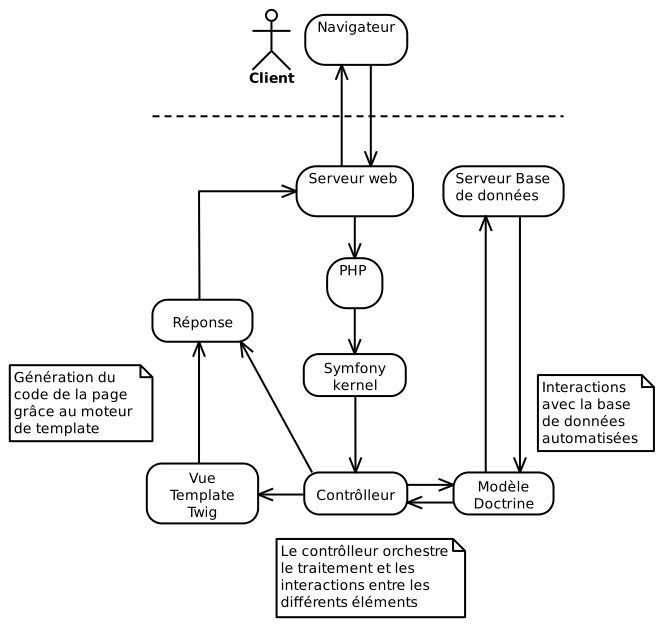
\includegraphics[width=0.7\linewidth]{pictures/mvc.png}
    %\caption{Architecture MVC dans Symfony}
\end{frame}

\begin{frame}
    \frametitle{Technologies utilisées}

    \begin{itemize}
        \item \textbf{Sass} : amélioration et structuration du CSS.
        \item Avantages de Sass :
              \begin{itemize}
                \item Variables et réutilisation de styles.
                \item Meilleure organisation du code CSS.
              \end{itemize}
        \item \textbf{JavaScript} : utilisé pour le jeu intégré au site.
    \end{itemize}
\end{frame}
